\documentclass{article}
\usepackage{setspace}
\usepackage[text={6.5in,8.5in},centering]{geometry}
\geometry{verbose,a4paper,tmargin=2.4cm,bmargin=2.4cm,lmargin=2.4cm,rmargin=2.4cm}
\usepackage{graphicx,amsmath,cases,multirow,appendix,graphicx,xcolor}

\setlength\parindent{0pt}

\newcommand{\note}[1]{\colorbox{gray!30}{#1}}
\newcommand{\ind}{\-\hspace{1cm}}

\begin{document}

\noindent\makebox[\textwidth][c]{\Large\bfseries Lecture 5 -- Density-independent deterministic growth}

\rule[0.5ex]{\linewidth}{1pt}
\begin{center}
	\note{Note: Probably won't finish MSY section.}
\end{center}
\rule[0.5ex]{\linewidth}{1pt}

\textbf{Concepts}: \\
\ind Population vs. Per capita growth rate \\
\ind Negative vs. Positive density-dependence \\
\ind Stable vs. Unstable fixed point equilibria \\
\ind Maximum Sustainable Yield (MSY)

\rule[0.5ex]{\linewidth}{1pt}

\begin{equation*}
	N_{t+1}=\lambda \cdot N_t = (1+r_d) N_t = N_t + r_d N_t
\end{equation*}
	Next year = previous year plus some per capita increment (proportion $r_d$ of previous year)\\
\ind	$r_d$ is discrete growth factor\\
		
Per capita increment is density-independent:
\begin{align*}
&	\frac{N_{t+1}}{N_t}=\lambda = 1+r_d \\
	\text{or equivalently...}&\\
&	\frac{N_{t+1}-N_t}{N_t}=r_d
\end{align*}

\note{When drawing, leave room for 3x3 = 9 graphs!}
\begin{center}
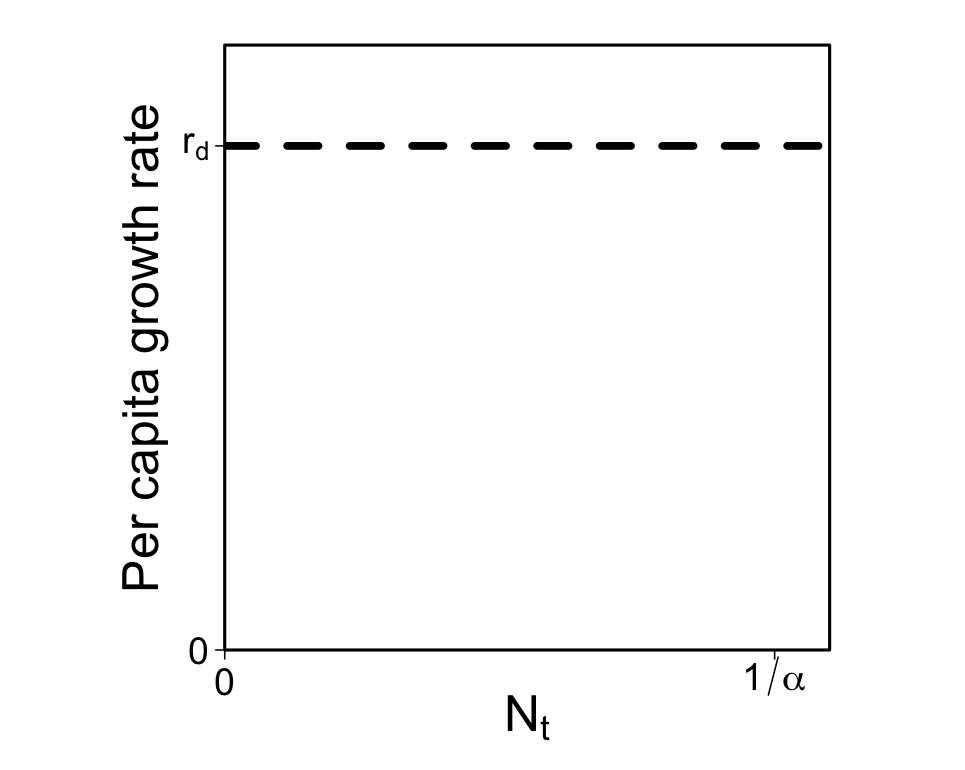
\includegraphics[width=5cm]{figs/percap.jpg}
\end{center}

\textbf{Now make per capita growth rate density-dependent:}\\
\emph{Realized} per capita growth increment $=r_d-\alpha N_t$
\begin{equation*}
	\frac{N_{t+1}}{N_t}=1+r_d-\alpha N_t
\end{equation*}
\ind $\alpha$ - per capita strength of density-dependence (self-limitation rate)\\
\begin{equation*}
\lim_{N_t \to 0} (r_d-\alpha N_t)=r_d
\end{equation*}

At what population size does realized per capita growth increment = 0?
\begin{align*}
	0&=r_d-\alpha N_t\\
	\alpha N_t &= r_d\\
	N_t&=\frac{r_d}{\alpha}\\
\end{align*}

\pagebreak

\note{Class Q:} Using $r_d-\alpha N_t$, plot realized per capita growth rate vs. $N_t$ for: \\
\ind density-independece
\ind positive density-dependence
\ind negative density-dependence.
\begin{center}
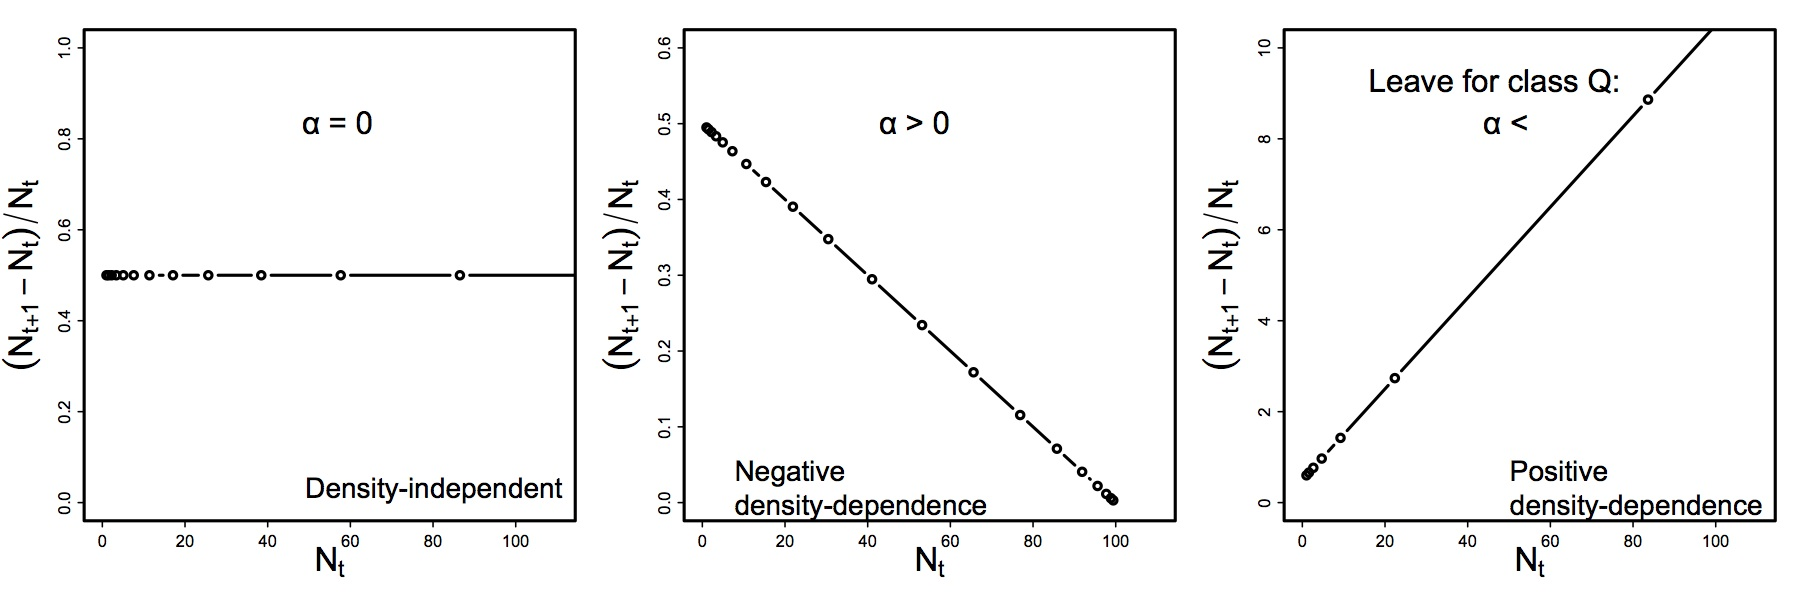
\includegraphics[width=10cm]{figs/densdep_percap.jpg}
\end{center}

\textbf{What do population dynamics look like?}

Plug into equation for population growth rate by replacing $r_d$ with $r_d-\alpha N_t$
\begin{align*}
	N_{t+1}=& N_t+(r_d-\alpha N_t)N_t &\;\;\;\;\text{(\emph{Discrete logistic growth eqn.})}\\
\text{Typically written with $K=\frac{r_d}{\alpha}$ for `carrying capacity':}&\\
	=  & N_t + \left(r_d-\frac{r_d}{K} N_t \right) N_t &\\
	=  & N_t + r_d\left(1-\frac{N_t}{K}\right) N_t &
\end{align*}
\note{Draw  one after the other:}\\
\note{Class Q:} What would positive density dependence look like?
\begin{center}
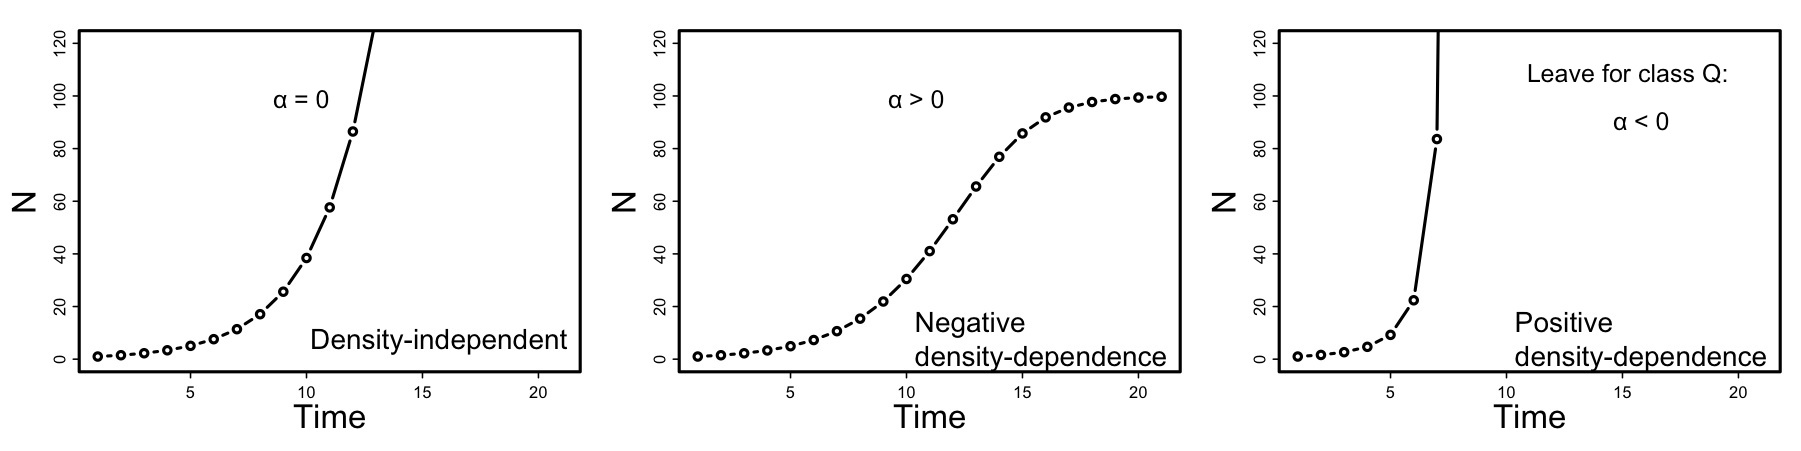
\includegraphics[width=12cm]{figs/densdep_popsize.jpg}
\end{center}



\note{Class Q:} Have you read Mark Kot's \emph{`Historical hiatus'}?\\
With what kind of density-dependence has the global human population been growing?\\
How is that possible?

\rule[0.5ex]{\linewidth}{1pt}

\textbf{Definition:}\\
The \emph{equilibrium} (a.k.a. steady state) abundance for the difference equation $N_{t+1} = F(N_t)$, is the value $N_t^*$ where $N_{t+1}=F(N^*_t)=N^*_t$ (i.e. population growth rate is zero.)\\
\ind (We will use $N^*$ to denote an equilibrium/steady-state.)

\rule[0.5ex]{\linewidth}{1pt}

\textbf{Class exercise 1:} Simulating logistic growth

\note{Walk through Part A of \emph{`Class5-Ex-LogisticGrowth.R'}}\\
\note{Allow students to explore.}\\


\note{Class Qs:} Where are the point equilibria?\\
\textbf{A:}\\
\ind \emph{Non-trivial point equilibrium:}\\
\begin{center}
	When $N_t^*=K$, growth rate $=0$, thus $N_{t+1}=N_t$.
\end{center}
\ind \emph{Trivial point equilibrium:}\\
\begin{center}
	When $N_t^*=0$, growth rate $=0$, thus $N_{t+1}=N_t$.
\end{center}

What happens with $N_t>K$?

Best way to see where equilibria is:\\ 
\ind Plot population-level growth rate, $(N_{t+1}-N_t)$ or $\frac{dN}{dt}$, as function of $N$


\pagebreak

\note{Class Q:} What does $N_{t+1}-N_t$ vs. $N_t$ look like?
\begin{center}
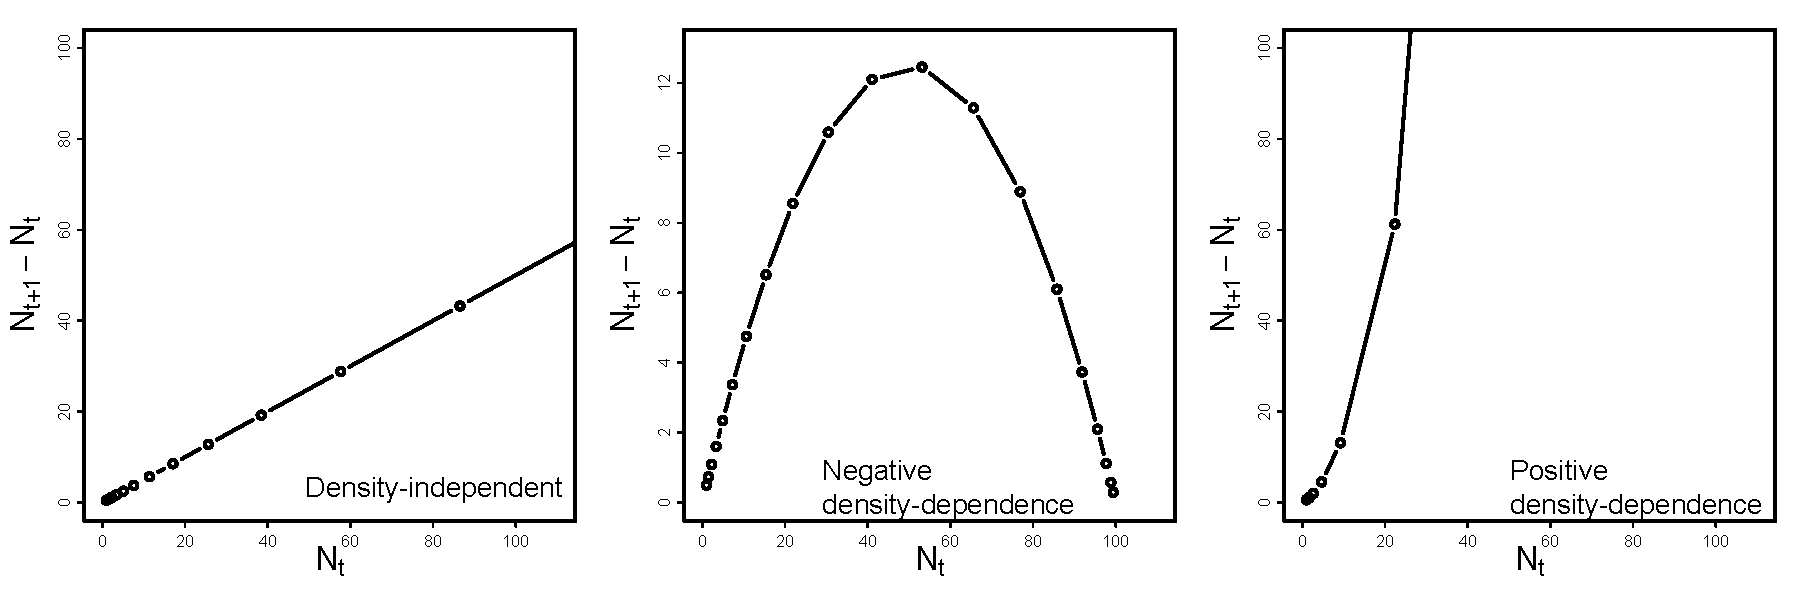
\includegraphics[width=12cm]{figs/densdep_popn.pdf}
\end{center}

At low $N$, few individuals to reproduce $\implies$ low population growth rate.\\
At high $N$, strong self-limitation $\implies$ low population growth rate.

\rule[0.5ex]{\linewidth}{1pt}

\textbf{Ball \& Cup analogy:}
\begin{center}
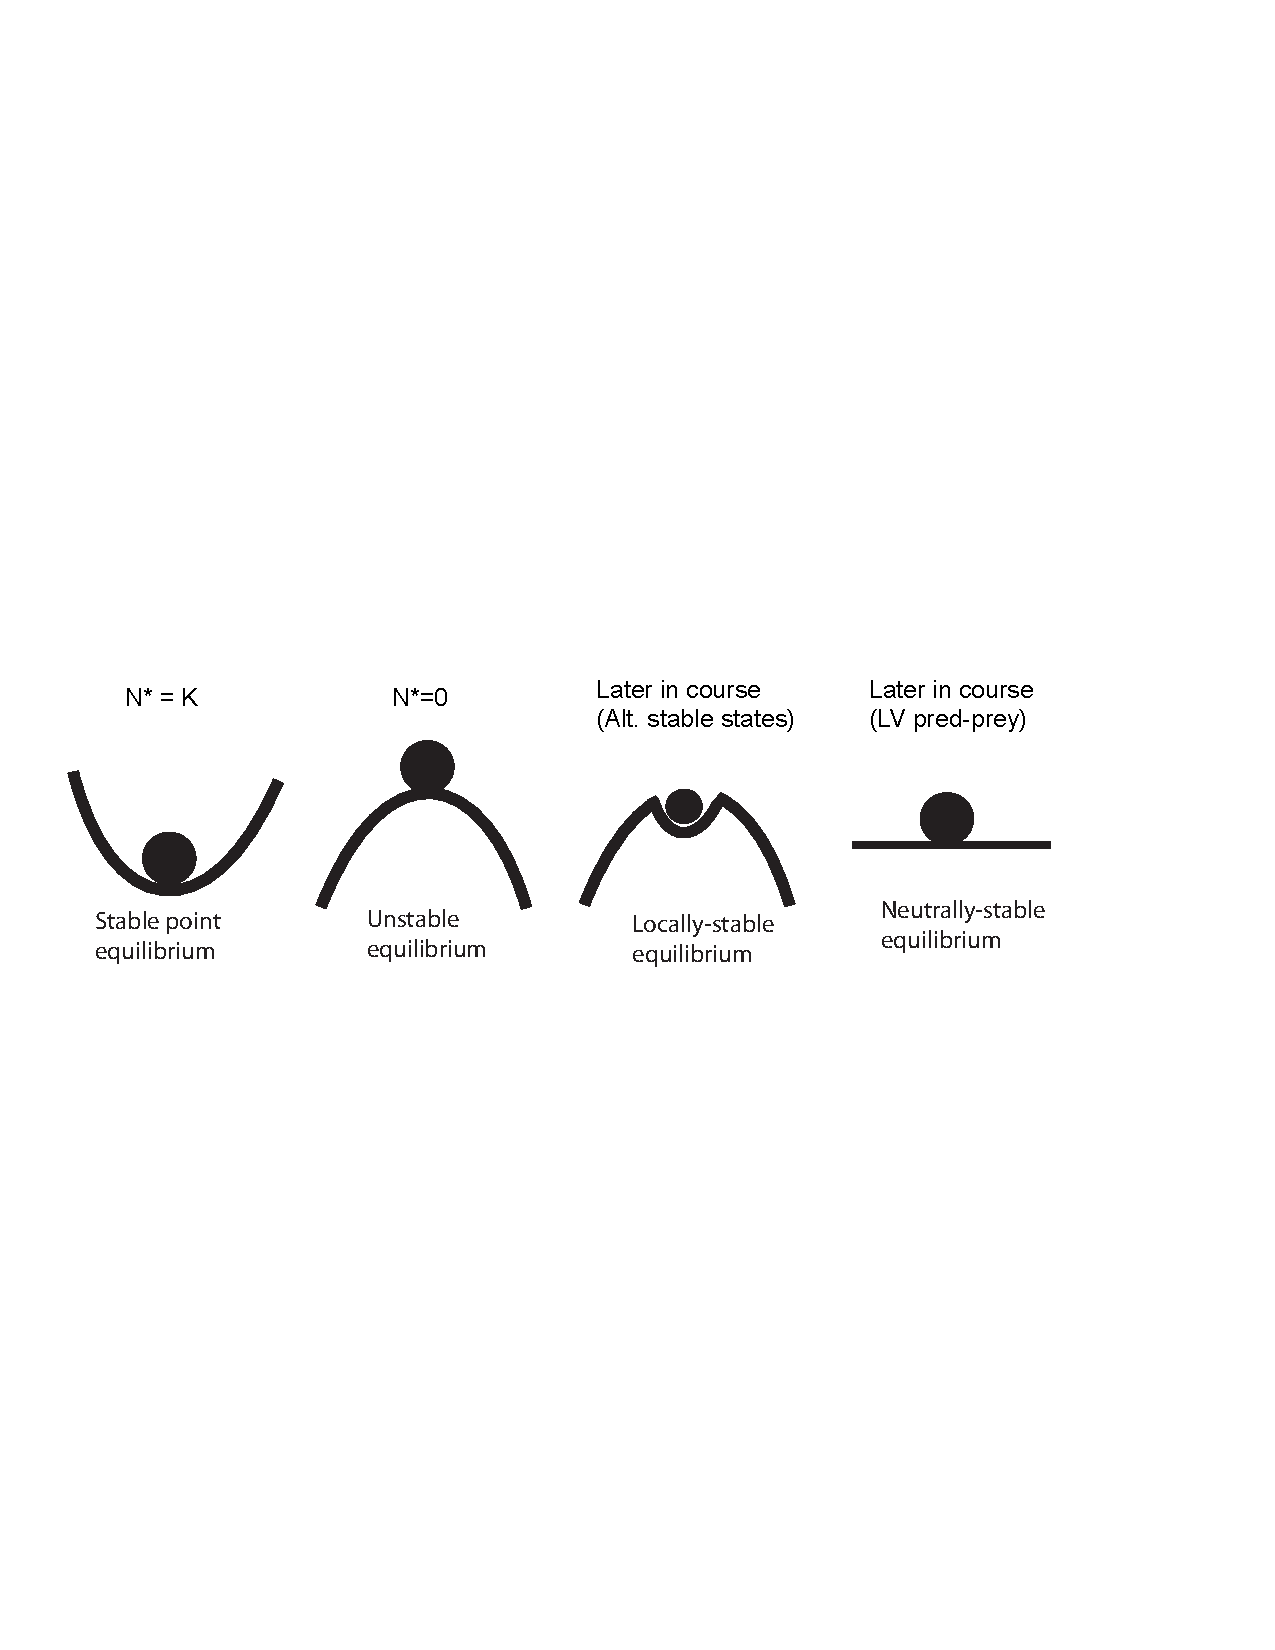
\includegraphics[width=12cm]{figs/ballcup.pdf}
\end{center}

\rule[0.5ex]{\linewidth}{1pt}

\textbf{Continuous logistic}

Recall: \textbf{Discrete geometric growth to continuous exponential growth}\\
\begin{center}
$N_{t+1}=(1+r_d)N_t$ converted to $N_t=N_0e^{rt}$\\
\end{center}
Differential equation solution:\\
\begin{equation*}
	\frac{d(N_0e^{rt})}{dt}=\frac{dN}{dt}=rN
\end{equation*}

\textbf{Discrete logistic:}\\
\begin{align*}
	N_{t+1}=N_t+r_d(1-\alpha N_t)N_t & \\ 
	\text{converts to}&
	\;\;\; N_t=\frac{N_0e^{rt}}{1+\alpha N_0 (e^{rt}-1)}\\
	\text{or equivalently}
	&\;\;\; N_t=\frac{K N_0}{N_0+(K-N_0)e^{-rt}}
\end{align*}
\note{Class Q:}  See if you can prove these equalities at home.\\
Hint: To go from 2nd to 1st, divide once by $\tfrac{K}{K}$ and multiply once by $\tfrac{N_0 e^{rt}}{N_0 e^{rt}}$.

\vspace{0.5cm}

\textbf{Differential solution:}
\begin{align*}
	\frac{dN}{dt}=rN-\alpha N^2=rN\left(1-\tfrac{N}{K}\right)
\end{align*}
the latter being attributed to Verhulst (1838)

\rule[0.5ex]{\linewidth}{1pt}

NOTE:  There are a number of other ways to represent density-dependent growth:\\
Ricker model (and extensions):
\begin{equation*}
	N_{t+1}=N_t e^{r(1-N_t /K)}
\end{equation*}
...which is a special case of the Beverton-Holt model
...which is a special case of the Hassell model.

\rule[0.5ex]{\linewidth}{1pt}

\pagebreak

\textbf{Definition:}\\
The steady state abundance for a differential equation $\frac{dN}{dt}=f(N)$ is the value $N^*$ where $f(N^*)=0$.\\
Population growth rate is zero.  System is at equilibrium.\\

For the logistic, there are two equilibria:\\
\ind Trivial equilibrium, $N^*=0$\\
\ind Non-trivial equilibrium, $N^*=K$.

\vspace{0.5cm}
\textbf{Solving for equilibria analytically:}
\begin{align*}
	\text{Step 1:  Set}\;\; f(N)=\frac{dN}{dt}=0&\\
	\text{Step 2:  Solve for}\;\;N^*&\\
	\frac{dN}{dt}&=rN\left(1-\frac{N}{K}\right)=0\\
	rN-\frac{rN^2}{K}&=0\\
	rN&=\frac{rN^2}{K}\\
	N&=\frac{N^2}{K}\\
	NK&=N^2\\
	N^*&=K
\end{align*}

\rule[0.5ex]{\linewidth}{1pt}

\textbf{Class Exercise 2} ODE-solvers and continuous logistic\\
\note{Walk through code}\\
\note{Class Q:} How do values of $r$, $K$, and $N_0$ affect the maximum value of $\frac{dN}{dt}$?

\begin{table}[h]
\centering
\begin{tabular}{|c|c|}
\hline
 \textbf{Parameter} & \textbf{Max. $\tfrac{dN}{dt}$} \\ 
 \hline
$N_0$ & doesn't affect \\ 
$r$ & increases \\ 
$K$ &  increases \\ 
\hline
\end{tabular} 
\end{table}

\begin{center}
	\textbf{With this knowledge you should be able to take Quiz 2.  So take it!}
\end{center}

\rule[0.5ex]{\linewidth}{1pt}

\pagebreak

\textbf{Maximum Sustainable Yield}

Where is maximum $\frac{dN}{dt}$?
\begin{equation*}
	\frac{dN}{dt}=rN\left(1-\frac{N}{K}\right)=rN-\frac{rN^2}{K}
\end{equation*}
Maximum occurs where slope $=0, \implies$ derivative with respect to $N$.

Step \#1:  Differentiate with respect to $N$
\begin{equation*}
	\frac{d\left(rN-\tfrac{rN^2}{K}\right)}{dN}=r-\frac{2rN}{K}
\end{equation*}
Step \#2: Set $=0$
\begin{equation*}
	r-\frac{2rN}{K}=0
\end{equation*}
Step \#3: Solve for $N$
\begin{align*}
&	2rN=rK\\
&	N=\frac{K}{2}
\end{align*}
\begin{center}
	\note{A:} Maximum population growth rate occurs at half the carrying capacity
\end{center}

\note{Q:} What is maximum possible population growth rate?

\note{A:} Plug in $\frac{K}{2}$ for $N$...
\begin{equation*}
	\frac{dN}{dt}=r\frac{K}{2}\left(1-\frac{K/2}{K}\right)=r\frac{K}{2}\left(1-\frac{1}{2}\right)=\frac{rK}{4}
\end{equation*}
\begin{center}
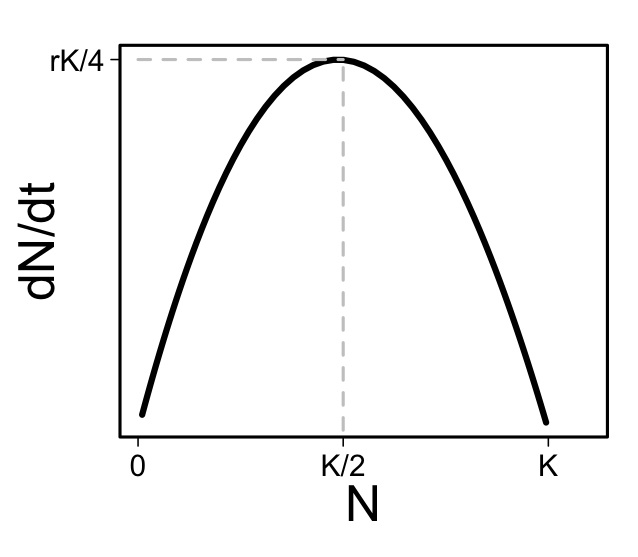
\includegraphics[width=4cm]{figs/dNdt.jpg}
\end{center}
\textbf{Context of harvest:}\\
$\frac{dN}{dt}$ vs. $N$  = Stock-recruitment function. \note{Replace axis labels on graph.}\\
\emph{Maximum Sustainable Yield} (MSY)\\
\ind Occurs when $N=\frac{K}{2}$ and produces harvestable biomass at rate $\frac{rK}{4}$.\\
\ind Over-fished when $N<\tfrac{K}{2}$\\
\ind Not over-fished when $N>\tfrac{K}{2}$.

\rule[0.5ex]{\linewidth}{1pt}

\textbf{Fixed-harvest scenario}
\begin{equation*}
	\frac{dN}{dt}=f(N)=rN\left(1-\frac{N}{K}\right)-H
\end{equation*}
\note{Class Q:} What are units of $H$? \note{A:} Individuals per time.
\vspace{0.5cm}

\emph{Solve for equilibria:}

Step \#1: Set $f(N)$ to $0$
\begin{equation*}
	\frac{dN}{dt}=rN\left(1-\frac{N}{K}\right)-H=0
\end{equation*}
Step \#2: Solve for $N^*$\\
\ind Trivial solution is $N^*=0$\\
\ind Rearrange to:
\begin{equation*}
	-\tfrac{r}{K}N^2+rN-H=0
\end{equation*}
\ind This is just like the quadratic equation...
\begin{equation*}
	ax^2 + bx + c = 0
\end{equation*}
\ind ...whose solution is...
\begin{equation*}
	x=\frac{-b \pm \sqrt{b^2-4ac}}{2a}
\end{equation*}
\ind Thus:
\begin{equation*}
	N^*=\frac{-r \pm \sqrt{r^2 - 4rH/K}}{-2r/K}=\frac{rK \pm \sqrt{r^2 K^2 - 4rKH}}{2r}
\end{equation*}
Thus model contains \emph{two} non-trivial solutions  and \emph{one} trivial solution!
\begin{center}
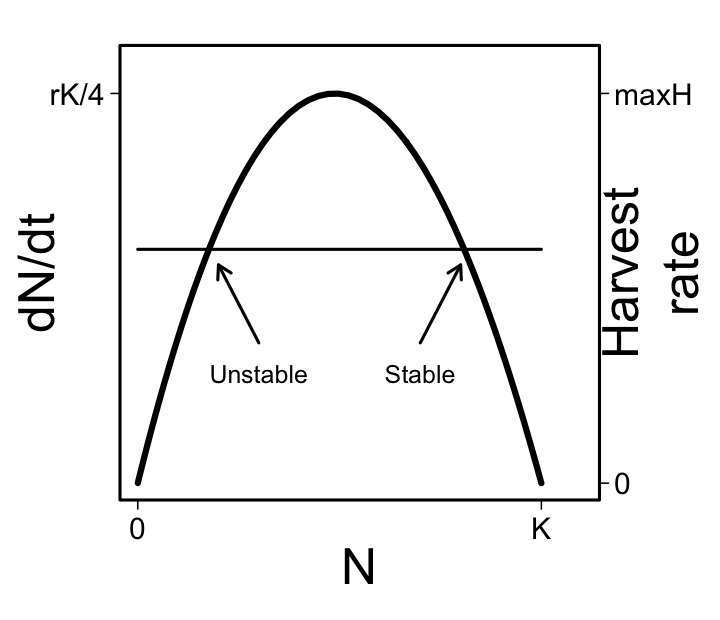
\includegraphics[width=4cm]{figs/dNdt_harvestquota.jpg}
\end{center}

Right-hand equilibrium is a stable fixed point.\\
\ind Stochastic fluctuations always return to feasible (positive) equilibrium.\\
Left-hand equilibrium is unstable.\\
\ind Positive fluctuation will send system to stable fixed point.\\
\ind Negative fluctuation will send system to extinction.\\

\rule[0.5ex]{\linewidth}{1pt}

\textbf{Problem for inferring MSY from real data}: \note{Show Fisheries figure.}

\rule[0.5ex]{\linewidth}{1pt}

\textbf{Fixed-effort harvest scenario}
\begin{equation*}
	\frac{dN}{dt}=f(N)=rN\left(1-\frac{N}{K}\right)-hN
\end{equation*}
\note{Class Q:} What are units of $h$? \note{A:} Individuals per individual (fraction of population) per time.
\vspace{0.5cm}

\emph{Solve for equilibria}\\
Step \#1: Set $f(N)$ to $0$
\begin{equation*}
	\frac{dN}{dt}=rN\left(1-\frac{N}{K}\right)-hN=0
\end{equation*}
Step \#2: Solve for $N^*$\\
\ind Trivial solution is $N^*=0$
\begin{equation*}
	N^*=\frac{rK-hK}{r}=\frac{(r-h)K}{r}
\end{equation*}
Thus model as \emph{one} trivial and \emph{one} non-trivial solution.\\
Visualize as slope = $h$
\begin{center}
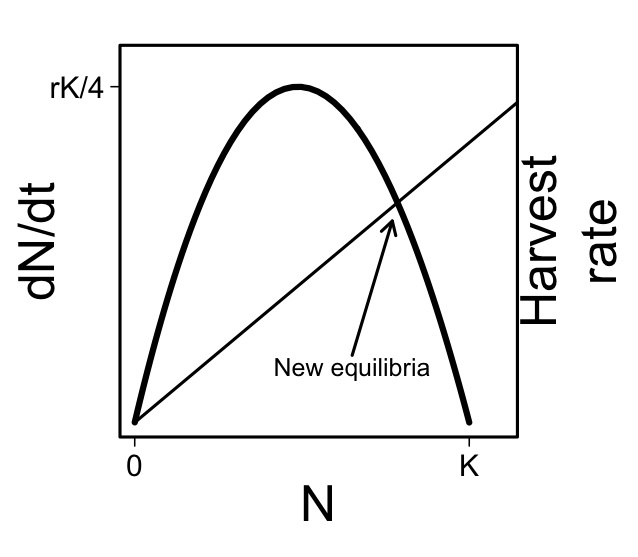
\includegraphics[width=4cm]{figs/dNdt_harvesteffort.jpg}
\end{center}
Non-trivial solution is always stable!\\
Also note intuitive interpretation:\\
\begin{equation*}
	N^*>0 \text{ as long as } r>h
\end{equation*}

\rule[0.5ex]{\linewidth}{1pt}

\pagebreak 

\textbf{Polynomial representation of $\frac{dN}{dt}$}

Recall: population size as function of time as polynomial
\begin{equation*}
	N(t)=\sum_{n=0}^\infty \beta_n t^n = \beta_0 + \beta_1 t + \beta_2 t^2 +...
\end{equation*}


Could also think of in terms of population growth 
\begin{align*}
&	\frac{dN}{dt}=f(N)=\sum_{n=0}^\infty \beta_n N^n
\end{align*}

such that exponential growth corresponds to ...
\begin{align*}
& 	\beta_0=0, \;\; \beta_1 = r, \;\; \beta_{n>1}=0\\
\end{align*}

and logistic growth corresponds to...
\begin{align*}
& 	\beta_0=0, \;\; \beta_1 = r, \;\; \beta_2 = -\frac{r}{K}, \;\; \beta_{n>2}=0\\
\end{align*}

\rule[0.5ex]{\linewidth}{1pt}
\rule[0.5ex]{\linewidth}{1pt}

\end{document}